% Options for packages loaded elsewhere
\PassOptionsToPackage{unicode}{hyperref}
\PassOptionsToPackage{hyphens}{url}
%
\documentclass[
]{article}
\usepackage{amsmath,amssymb}
\usepackage{lmodern}
\usepackage{ifxetex,ifluatex}
\ifnum 0\ifxetex 1\fi\ifluatex 1\fi=0 % if pdftex
  \usepackage[T1]{fontenc}
  \usepackage[utf8]{inputenc}
  \usepackage{textcomp} % provide euro and other symbols
\else % if luatex or xetex
  \usepackage{unicode-math}
  \defaultfontfeatures{Scale=MatchLowercase}
  \defaultfontfeatures[\rmfamily]{Ligatures=TeX,Scale=1}
\fi
% Use upquote if available, for straight quotes in verbatim environments
\IfFileExists{upquote.sty}{\usepackage{upquote}}{}
\IfFileExists{microtype.sty}{% use microtype if available
  \usepackage[]{microtype}
  \UseMicrotypeSet[protrusion]{basicmath} % disable protrusion for tt fonts
}{}
\makeatletter
\@ifundefined{KOMAClassName}{% if non-KOMA class
  \IfFileExists{parskip.sty}{%
    \usepackage{parskip}
  }{% else
    \setlength{\parindent}{0pt}
    \setlength{\parskip}{6pt plus 2pt minus 1pt}}
}{% if KOMA class
  \KOMAoptions{parskip=half}}
\makeatother
\usepackage{xcolor}
\IfFileExists{xurl.sty}{\usepackage{xurl}}{} % add URL line breaks if available
\IfFileExists{bookmark.sty}{\usepackage{bookmark}}{\usepackage{hyperref}}
\hypersetup{
  pdftitle={Using pandoc-ling},
  pdfauthor={Michael Cysouw},
  hidelinks,
  pdfcreator={LaTeX via pandoc}}
\urlstyle{same} % disable monospaced font for URLs
\usepackage{graphicx}
\makeatletter
\def\maxwidth{\ifdim\Gin@nat@width>\linewidth\linewidth\else\Gin@nat@width\fi}
\def\maxheight{\ifdim\Gin@nat@height>\textheight\textheight\else\Gin@nat@height\fi}
\makeatother
% Scale images if necessary, so that they will not overflow the page
% margins by default, and it is still possible to overwrite the defaults
% using explicit options in \includegraphics[width, height, ...]{}
\setkeys{Gin}{width=\maxwidth,height=\maxheight,keepaspectratio}
% Set default figure placement to htbp
\makeatletter
\def\fps@figure{htbp}
\makeatother
\setlength{\emergencystretch}{3em} % prevent overfull lines
\providecommand{\tightlist}{%
  \setlength{\itemsep}{0pt}\setlength{\parskip}{0pt}}
\setcounter{secnumdepth}{5}
\usepackage{langsci-gb4e}
\usepackage[noparens]{nnext}
\usepackage{chngcntr}
\counterwithin{xnumi}{section}
\ifluatex
  \usepackage{selnolig}  % disable illegal ligatures
\fi

\title{Using pandoc-ling}
\author{Michael Cysouw}
\date{}

\begin{document}
\maketitle

{
\setcounter{tocdepth}{3}
\tableofcontents
}
\hypertarget{pandoc-ling}{%
\section{pandoc-ling}\label{pandoc-ling}}

\emph{Michael Cysouw}
\textless{}\href{mailto:cysouw@mac.com}{\nolinkurl{cysouw@mac.com}}\textgreater{}

A Pandoc filter for linguistic examples

tl;dr

\begin{itemize}
\tightlist
\item
  Easily write linguistic examples including basic interlinear glossing.
\item
  Let numbering and cross-referencing be done for you.
\item
  Export to (almost) any format of your wishes for final polishing.
\item
  As an example, check out this readme in
  \href{https://gitcdn.link/repo/cysouw/pandoc-ling/main/readme\%20conversions/readme2.html}{HTML}
  or
  \href{https://gitcdn.link/repo/cysouw/pandoc-ling/main/readme\%20conversions/readme2_linguex.pdf}{Latex}.
\end{itemize}

\hypertarget{rationale}{%
\section{Rationale}\label{rationale}}

In the field of linguistics there is an outspoken tradition to format
example sentences in research papers in a very specific way. In the
field, it is a perennial problem to get such example sentences to look
just right. Within Latex, there are numerous packages to deal with this
problem (e.g.~covington, linguex, gb4e, expex, etc.). Depending on your
needs, there is some Latex solution for almost everyone. However, these
solutions in Latex are often cumbersome to type, and they are not
portable to other formats. Specifically, transfer between Latex, html,
docx, odt or epub would actually be highly desirable. Such transfer is
the hallmark of \href{https://pandoc.org}{Pandoc}, a tool by John
MacFarlane that provides conversion between these (and many more)
formats.

Any such conversion between text-formats naturally never works
perfectly: every text-format has specific features that are not
transferable to other formats. A central goal of Pandoc (at least in my
interpretation) is to define a set of shared concepts for text-structure
(a `common denominator' if you will, but surely not `least'!) that can
then be mapped to other formats. In many ways, Pandoc tries (again) to
define a set of logical concepts for text structure (`semantic markup'),
which can then be formatted by your favourite typesetter. As long as you
stay inside the realm of this `common denominator' (in practice that
means Pandoc's extended version of Markdown/CommonMark), conversion
works reasonably well (think 90\%-plus).

Building on John Gruber's
\href{https://daringfireball.net/projects/markdown/syntax}{Markdown
philosophy}, there is a strong urge here to learn to restrain oneself
while writing, and try to restrict the number of layout-possibilities to
a minimum. In this sense, with \texttt{pandoc-ling} I propose a
Markdown-structure for linguistic examples that is simple, easy to type,
easy to read, and portable through the Pandoc universe by way of an
extension mechanism of Pandoc, called a `Pandoc Lua Filter'. This
extension will not magically allow you to write every linguistic example
thinkable, but my guess is that in practice the present proposal covers
the majority of situations in linguistic publications (think 90\%-plus).
As an example (and test case) I have included automatic conversions into
various formats in this repository (chech them out to get an idea of the
strengths and weaknesses of this approach).

\hypertarget{the-basic-structure-of-a-linguistic-example}{%
\section{The basic structure of a linguistic
example}\label{the-basic-structure-of-a-linguistic-example}}

Basically, a linguistic examples consists of 6 possible building blocks,
of which only the number and at least one example line are necessary.
The space between the building blocks is kept as minimal as possible
without becoming cramped. When (optional) building blocks are not
included, then the other blocks shift left and up (only exception: a
preamble without labels is not shifted left completely, but left-aligned
with the example, not with the judgement).

\begin{itemize}
\tightlist
\item
  \textbf{Number}: Running tally of all examples in the work, possibly
  restarting at chapters or other major headings. Typically between
  round brackets, possibly with a chapter number added before in long
  works, e.g.~example (7.26). Aligned top-left, typically left-aligned
  to main text margin.
\item
  \textbf{Preamble}: Optional information about the content/kind of
  example. Aligned top-left: to the top with the number, to the left
  with the (optional) label. When there is no label, then preamble is
  aligned with the example, not with the judgment.
\item
  \textbf{Label}: Indices for sub-examples. Only present when there are
  more than one example grouped together inside one numbered entity.
  Typically these sub-example labels use latin letters followed by a
  full stop. They are left-aligned with the preamble, and each label is
  top-aligned with the top-line of the corresponding example (important
  for longer line-wrapped examples).
\item
  \textbf{Judgment}: Examples can optionally have grammaticality
  judgments, typically symbols like **?!* sometimes in superscript
  relative to the corresponding example. judgements are right-aligned to
  each other, typically with only minimal space to the left-aligned
  examples.
\item
  \textbf{Line example}: A minimal linguistic example has at least one
  line example, i.e.~an utterance of interest. Building blocks in
  general shift left and up when other (optional) building blocks are
  not present. Minimally, this results in a number with one line
  example.
\item
  \textbf{Interlinear example}: A complex structure typically used for
  examples from languages unknown to most readers. Consist of three or
  four lines that are left-aligned:

  \begin{itemize}
  \tightlist
  \item
    \textbf{Header}: An optional header is typically used to display
    information about the language of the example, including literature
    references. When not present, then all other lines from the
    interlinear example shift upwards.
  \item
    \textbf{Source}: The actual language utterance, often typeset in
    italics. This line is internally separated at spaces, and each
    sub-block is left-aligned with the corresponding sub-blocks of the
    gloss.
  \item
    \textbf{Gloss}: Explanation of the meaning of the source, often
    using abbreviations in small caps. This line is internally separated
    at spaces, and each block is left-aligned with the block from
    source.
  \item
    \textbf{Translation}: Free translation of the source, typically
    quoted. Not separated in blocks, but freely extending to the right.
    Left-aligned with the other lines from the interlinear example.
  \end{itemize}
\end{itemize}

\begin{figure}
\centering
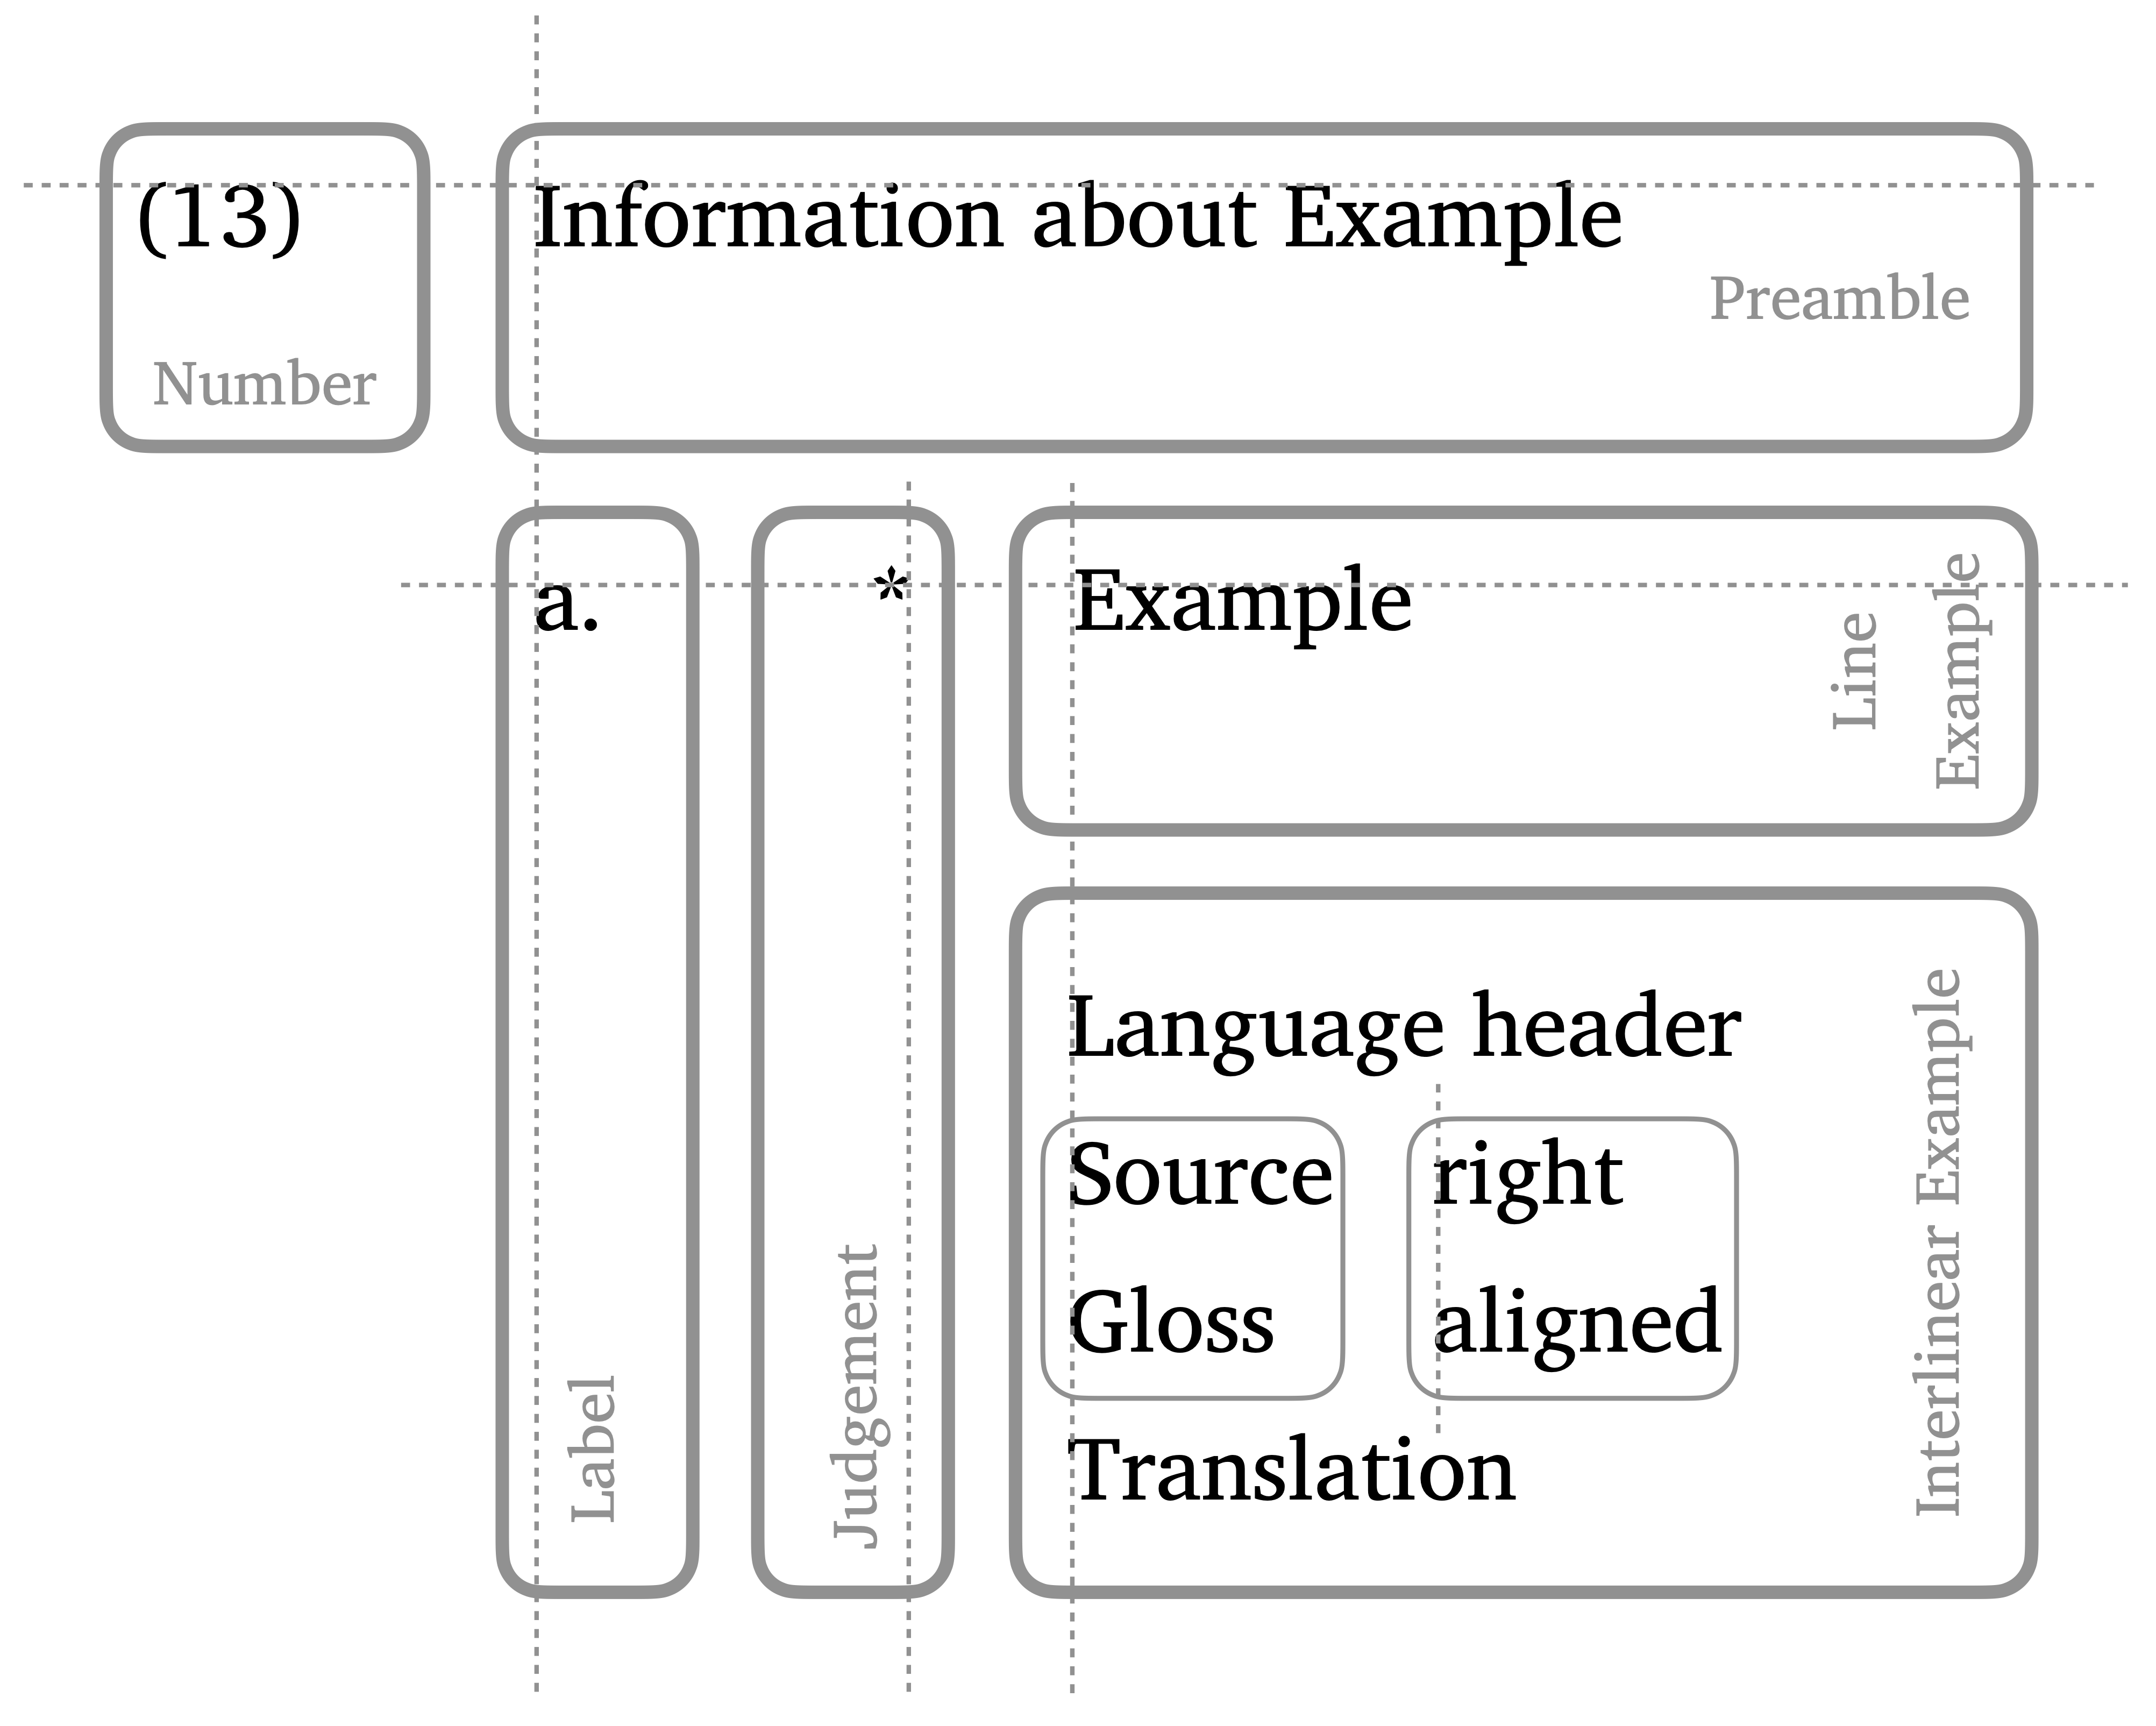
\includegraphics{figure/ExampleStructure.png}
\caption{The structure of a linguistic example.}
\end{figure}

There are of course much more possibilities to extend the structure of a
linguistic examples, like third or fourth subdivisions of labels (often
using small roman numerals as a third level) or multiple glossing lines
in the interlinear example. Also, the content of the header is sometimes
found right-aligned to the right of the interlinear example (language
into to the top, reference to the bottom). All such options are
currently not supported by \texttt{pandoc-ling}.

Under the hood, this structure is prepared by \texttt{pandoc-ling} as a
table. Tables are reasonably well transcoded to different document
formats. Specific layout considerations mostly have to be set manually.
Alignment of the text should work in most exports. Some \texttt{CSS}
styling is proposed by \texttt{pandoc-ling}, but can of course be
overruled. For latex (and beamer) special output is prepared using
various available latex packages (see options, below).

\hypertarget{introducing-pandoc-ling}{%
\section{\texorpdfstring{Introducing
\texttt{pandoc-ling}}{Introducing pandoc-ling}}\label{introducing-pandoc-ling}}

\hypertarget{editing-linguistic-examples}{%
\subsection{Editing linguistic
examples}\label{editing-linguistic-examples}}

To include a linguistic example in Markdown \texttt{pandoc-ling} uses
the \texttt{div} structure, which is indicated in Pandoc-Markdown by
typing three colons at the start and three colons at the end. To
indicate the \texttt{class} of this \texttt{div} the letters `ex' (for
`example') should be added after the top colons (with or without space
in between). This `ex'-class is the signal for \texttt{pandoc-ling} to
start processing such a \texttt{div}. The numbering of these examples
will be inserted by \texttt{pandoc-ling}.

Empty lines can be added inside the \texttt{div} for visual pleasure, as
they mostly do not have an influence on the output. Exception: do
\emph{not} use empty lines between unlabelled line examples. Multiple
lines of text can be used (without empty lines in between), but they
will simply be interpreted as one sequential paragraph.

\begin{verbatim}
::: ex
This is the most basic structure of a linguistic example. 
:::
\end{verbatim}

\ea \judgewidth{} \label{ling-ex:4.1} 
  This is the most basic structure of a linguistic example.
\z

Alternatively, the \texttt{class} can be put in curled brackets (and
then a leading full stop is necessary before \texttt{ex}). Inside these
brackets more attributes can be added (separated by space), for example
an id, using a hash, or any attribute=value pairs that should apply to
this example. Currently there is only one attribute implemented
(\texttt{formatGloss}), but in principle it is possible to add more
attributes that can be used to fine-tune the typesetting of the example.

\begin{verbatim}
::: {#id .ex formatGloss=false}

This is a multi-line example.
But that does not mean anything for the result
All these lines are simply treated as one paragraph.
They will become one example with one number.

:::
\end{verbatim}

\ea \judgewidth{} \label{id} 
  This is a multi-line example. But that does not mean anything for the
result All these lines are simply treated as one paragraph. They will
become one example with one number.
\z

A preamble can be added by inserting an empty line between preamble and
example. The same considerations about multiple text-lines apply.

\begin{verbatim}
:::ex
Preamble

This is an example with a preamble.
:::
\end{verbatim}

\ea \judgewidth{} \label{ling-ex:4.3} Preamble\\
  This is an example with a preamble.
\z

Sub-examples with labels are entered by starting each sub-example with a
small latin letter and a full stop. Empty lines between labels are
allowed. Subsequent lines without labels are treated as one paragraph.
Empty lines \emph{not} followed by a label with a full stop will result
in errors.

\begin{verbatim}
:::ex
a. This is the first example.
b. This is the second.
a. The actual letters are not important, `pandoc-ling` will put them in order.

e. Empty lines are allowed between labelled lines
Subsequent lines are again treated as one sequential paragraph.
:::
\end{verbatim}

\ea \judgewidth{} \label{ling-ex:4.4} 
  \ea [] { This is the first example. }
  \ex [] { This is the second. }
  \ex [] { The actual letters are not important, \texttt{pandoc-ling}
will put them in order. }
  \ex [] { Empty lines are allowed between labelled lines Subsequent
lines are again treated as one sequential paragraph. }
  \z
\z

A labelled list can be combined with a preamble.

\begin{verbatim}
:::ex
Any nice description here

a. one example sentence.
b. two
c. three
:::
\end{verbatim}

\ea \judgewidth{} \label{ling-ex:4.5} Any nice description here
  \ea [] { one example sentence. }
  \ex [] { two }
  \ex [] { three }
  \z
\z

Grammaticality judgements should be added before an example, and after
an optional label, separated from both by spaces (though four spaces in
a row should be avoided, that could lead to layout errors). To indicate
that any sequence of symbols is a judgements, prepend the judgement with
a caret \texttt{\^{}}. Alignment will be figured out by
\texttt{pandoc-ling}.

\begin{verbatim}
:::ex
Throwing in a preamble for good measure

a. ^* This traditionally signals ungrammaticality.
b. ^? Question-marks indicate questionable grammaticality.
c. ^^whynot?^ But in principle any sequence can be used (here even in superscript).
d. However, such long sequences sometimes lead to undesirable effects in the layout.
:::
\end{verbatim}

\ea \judgewidth{whynot?} \label{ling-ex:4.6} Throwing in a preamble for
good measure
  \ea [*] { This traditionally signals ungrammaticality. }
  \ex [?] { Question-marks indicate questionable grammaticality. }
  \ex [\textsuperscript{whynot?}] { But in principle any sequence can be
used (here even in superscript). }
  \ex [] { However, such long sequences sometimes lead to undesirable
effects in the layout. }
  \z
\z

A minor detail is the alignment of a single example with a preamble and
grammaticality judgements. In this case it looks better for the preamble
to be left aligned with the example and not with the judgement.

\begin{verbatim}
:::ex
Here is a special case with a preamble

^^???^ With a singly questionably example.
Note the alignment! Especially with this very long example
that should go over various lines in the output.
:::
\end{verbatim}

\ea \judgewidth{???} \label{ling-ex:4.7} Here is a special case with a
preamble\\
  \textsuperscript{???}With a singly questionably example. Note the
alignment! Especially with this very long example that should go over
various lines in the output.
\z

\hypertarget{interlinear-examples}{%
\subsection{Interlinear examples}\label{interlinear-examples}}

For interlinear examples with aligned source and gloss, the structure of
a \texttt{lineblock} is used, starting the lines with a vertical line
\texttt{\textbar{}}. There should always be four vertical lines (for
header, source, gloss and translation, respectively), although the
content after the first vertical line can be empty. The source and gloss
lines are separated at spaces, and all parts are right-aligned. If you
want to have a space that is not separated, you will have to `protect'
the space, either by putting a backslash before the space, or by
inserting a non-breaking space instead of a normal space (either type
\texttt{\&nbsp;} or insert an actual non-breaking space, i.e.~unicode
character \texttt{U+00A0}).

\begin{verbatim}
:::ex
| Dutch (Germanic)
| Deze zin is in het nederlands.
| DEM sentence AUX in DET dutch.
| This sentence is dutch.
:::
\end{verbatim}

\ea [] { \judgewidth{} \label{ling-ex:4.8} 
       Dutch (Germanic)\\
  \gll Deze zin is in het nederlands. \\
       DEM sentence AUX in DET dutch. \\
  \glt This sentence is dutch. }
\z

An attempt is made to format interlinear examples when the option
\texttt{formatGloss=true} is added. This will:

\begin{itemize}
\tightlist
\item
  remove formatting from the source and set everything in italics,
\item
  remove formatting from the gloss and set sequences (\textgreater1) of
  capitals and numbers into small caps (note that the positioning of
  small caps on web pages is
  \href{https://iamvdo.me/en/blog/css-font-metrics-line-height-and-vertical-align}{highly
  complex}),
\item
  a tilde \texttt{\textasciitilde{}} between spaces in the gloss is
  treated as a shortcut for an empty gloss (internally, the sequence
  \texttt{space-tilde-space} is replaced by
  \texttt{space-space-nonBreakingSpace-space-space}),
\item
  consistently put translations in single quotes, possibly removing
  other quotes.
\end{itemize}

\begin{verbatim}
::: {.ex formatGloss=true}
| Dutch (Germanic)
| Deze zin is in het nederlands.
| DEM sentence AUX in DET dutch.
| This sentence is dutch.
:::
\end{verbatim}

\ea [] { \judgewidth{} \label{ling-ex:4.9} 
       Dutch (Germanic)\\
  \gll \emph{Deze} \emph{zin} \emph{is} \emph{in} \emph{het}
\emph{nederlands.} \\
       \textsc{dem} sentence \textsc{aux} in \textsc{det} dutch. \\
  \glt `This sentence is dutch.' }
\z

The results of such formatting will not always work, but it seems to be
quite robust in my testing. The next example brings everything together:

\begin{itemize}
\tightlist
\item
  a preamble,
\item
  labels, both for single lines and for interlinear examples,
\item
  interlinear examples start on a new line immediately after the
  letter-label,
\item
  grammaticality judgements with proper alignment,
\item
  when the header of an interlinear example is left out, everything is
  shifted up,
\item
  The formatting of the interlinear is harmonised.
\end{itemize}

\begin{verbatim}
::: {.ex formatGloss=true}
Completely superfluous preamble, but it works ...

a. Mixing single line examples with interlinear examples.
a. This is of course highly unusal.
Just for this example, let's add some extra material in this example.

a.
| Dutch (Germanic) Note the grammaticality judgement!
| ^^:-)^ Deze zin is (dit\ is&nbsp;test) nederlands.
| DEM sentence AUX ~ dutch.
| This sentence is dutch.

b.
|
| Deze tweede zin heeft geen header.
| DEM second sentence have.3SG.PRES no header.
| This second sentence does not have a header.
:::
\end{verbatim}

\ea \judgewidth{:-)} \label{ling-ex:4.10} Completely superfluous
preamble, but it works \ldots{}
  \ea [] { Mixing single line examples with interlinear examples. }
  \ex [] { This is of course highly unusal. Just for this example, let's
add some extra material in this example. }
  \ex [\textsuperscript{:-)}] { 
       Dutch (Germanic) Note the grammaticality judgement!\\
  \gll \emph{Deze} \emph{zin} \emph{is} \emph{(dit~is~test)}
\emph{nederlands.} \\
       \textsc{dem} sentence \textsc{aux}  ~  dutch. \\
  \glt `This sentence is dutch.' }
  \ex [] { 
  \gll \emph{Deze} \emph{tweede} \emph{zin} \emph{heeft} \emph{geen}
\emph{header.} \\
       \textsc{dem} second sentence have.\textsc{3sg}.\textsc{pres} no
header. \\
  \glt `This second sentence does not have a header.' }
  \z
\z

\hypertarget{cross-referencing-examples}{%
\subsection{Cross-referencing
examples}\label{cross-referencing-examples}}

The examples are automatically numbered by \texttt{pandoc-ling}.
Cross-references to examples can be made by using the \texttt{{[}@ID{]}}
format (used by Pandoc for citations). When an example has an explicit
identifier (like \texttt{\#test} in the next example), then a reference
can be made to this example with \texttt{{[}@test{]}}, leading to
(\ref{test}) when formatted.

\begin{verbatim}
::: {#test .ex}
This is a test
:::
\end{verbatim}

\ea \judgewidth{} \label{test} 
  This is a test
\z

Inspired by the \texttt{linguex}-approach, you can also use the keywords
\texttt{Next} or \texttt{Last} to refer to the next or the last example,
e.g.~\texttt{{[}@Last{]}} will be formatted as (\ref{test}). By doubling
the capitals to \texttt{NNext} or \texttt{LLast} reference to the
next/last-but-one can be made. Actually, the number of starting capitals
can be repeated at will in \texttt{pandoc-ling}, so something like
\texttt{{[}@LLLLLLLLast{]}} will also work. It will be formatted as
(\ref{ling-ex:4.4}) after the processing of \texttt{pandoc-ling}.
Needless to say that in such a situation an explicit identifier would be
a better choice.

Referring to sub-examples can be done by manually adding a suffix into
the cross reference, simply separated from the identifier by a space.
For example, \texttt{{[}@LLast~c{]}} will refer to the third sub-example
of the last-but-one example. Formatted this will look like this:
(\ref{ling-ex:4.10}\,c), smile! However, note that the ``c'' has to be
manually determined. It is simply a literal suffix that will be copied
into the cross-reference. Something like \texttt{{[}@LLast\ Ha1l0{]}}
will work also, leading to (\ref{ling-ex:4.10}\,Ha1l0) when formatted
(which is of course nonsensical).

\hypertarget{options-of-pandoc-ling}{%
\subsection{\texorpdfstring{Options of
\texttt{pandoc-ling}}{Options of pandoc-ling}}\label{options-of-pandoc-ling}}

\hypertarget{global-options}{%
\subsubsection{Global options}\label{global-options}}

The following global options are available with \texttt{pandoc-ling}.
These can be added to the
\href{https://pandoc.org/MANUAL.html\#metadata-blocks}{Pandoc metadata}.
An example of such metadata can be found at the bottom of this
\texttt{readme} in the form of a YAML-block. Pandoc allows for various
methods to provide metadata (see the link above).

\begin{itemize}
\tightlist
\item
  \textbf{\texttt{formatGloss}} (boolean, default \texttt{false}):
  should all interlinear examples be consistently formatted? If you use
  this option, you can simply use capital letters for abbreviations in
  the gloss, and they will be changed to small caps. The source line is
  set to italics, and the translations is put into single quotes.
\item
  \textbf{\texttt{xrefSuffixSep}} (string, defaults to no-break-space):
  When cross references have a suffix, how should the separator be
  formatted? The defaults `no-break-space' is a safe options, but I
  personally like a `thin space' better (Unicode \texttt{U+2009}), but
  symbol does not work with many fonts, and might lead to errors. For
  Latex typesetting, all space-like symbols are converted to a Latex
  thin space \texttt{\textbackslash{},}.
\item
  \textbf{\texttt{restartAtChapter}} (boolean, default \texttt{false}):
  should the counting restart for each chapter? Actually, when
  \texttt{true} this setting will restart the counting at the highest
  heading level, which for various output formats can be set by the
  Pandoc option \texttt{top-level-division}. Depending on your Latex
  setup, an explicit entry \texttt{top-level-division:\ chapter} might
  be necessary in your metadata.
\item
  \textbf{\texttt{addChapterNumber}} (boolean, default \texttt{false}):
  should the chapter (= highest heading level) number be added to the
  number of the example? In most formats this automatically implies
  \texttt{restartAtChapter:\ true}. In most Latex situations this only
  works in combination with a \texttt{documentclass:\ book}.
\item
  \textbf{\texttt{latexPackage}} (one of: \texttt{linguex},
  \texttt{gb4e}, \texttt{langsci-gb4e}, \texttt{expex}, default
  \texttt{linguex}): Various options for converting examples to Latex
  packages that typeset linguistic examples. None of the conversions
  works perfectly, though in should work in most normal situations
  (think 90\%-plus). It might be necessary to first convert to
  \texttt{Latex}, correct the output, and then typeset separately with a
  latex compiler like \texttt{xelatex}. Using the direct option insider
  Pandoc might also work in many situations. Export to
  \textbf{\texttt{beamer}} seems to work reasonably well with the
  \texttt{gb4e} package. All others have artefacts or errors.
\end{itemize}

\hypertarget{local-options}{%
\subsubsection{Local options}\label{local-options}}

Local options are options that can be set for each individual example.
The \texttt{formatGloss} option can be used to have an individual
example be formatted differently from the global setting. For example,
when the global setting is \texttt{formatGloss:\ true} in the metadata,
then adding \texttt{formatGloss=false} in the curly brackets of a
specific example will block the formatting. This is especially useful
when the automatic formatting does not give the desired result.

If you want to add something else (not a linguistic example) in a
numbered example, then there is the local option \texttt{noFormat=true}.
An attempt will be made to try and do a reasonable layout. Multiple
paragraphs will simply we taken as is, and the number will be put in
front. In HTML the number will be centred. It is usable for an
incidental mathematical formula.

\begin{verbatim}
::: {.ex noFormat=true}
$$\sum_{x=1}^{n}{x}=\frac{x^2-x}{2}$$
:::
\end{verbatim}

\ea \judgewidth{} \label{ling-ex:4.12} 
  \[\sum_{x=1}^{n}{x}=\frac{x^2-x}{2}\]\\
  
\z

\hypertarget{issues-with-pandoc-ling}{%
\subsection{\texorpdfstring{Issues with
\texttt{pandoc-ling}}{Issues with pandoc-ling}}\label{issues-with-pandoc-ling}}

\begin{itemize}
\tightlist
\item
  Manually provided identifiers for examples should not be purely
  numerical (so do not use e.g.~\texttt{\#5789}). In some situation this
  interferes with the setting of the cross-references.
\item
  Because the cross-references use the same structure as citations in
  Pandoc, the processing of citations (by \texttt{citeproc}) should be
  performed \textbf{after} the processing by \texttt{pandoc-ling}.
  Further,
  \href{https://github.com/lierdakil/pandoc-crossref}{\texttt{pandoc-crossref}},
  another Pandoc extension for numbering figures and other captions,
  also uses the same system. From experience, it seems safer to put
  \texttt{pandoc-crossref} \textbf{before} \texttt{pandoc-ling} in the
  order of processing (though I have no idea why).
\item
  Interlinear examples will will not wrap at the end of the page. There
  is no solution yet for longer examples that are longer than the size
  of the page.
\item
  When exporting to \texttt{docx} there is a problem because there are
  paragraphs inserted after tables, which adds space in lists with
  multiple interlinear examples. This is
  \href{https://answers.microsoft.com/en-us/msoffice/forum/msoffice_word-mso_windows8-mso_2013_release/how-to-remove-extra-paragraph-after-table/995b3811-9f55-4df1-bbbc-9f672b1ad262}{by
  design}. The official solution is to set font-size to 1 for this
  paragraph inside MS Word.
\item
  Multi-column cells are crucial for \texttt{pandoc-ling} to work
  properly. These are only introduced in new table format with Pandoc
  2.10 (so older Pandoc version are not supported). Also note that these
  structures are not yet exported to all formats, e.g.~it will not be
  displayed correctly in \texttt{docx}. However, this is currently an
  area of active development
\item
  \texttt{langsci-gb4e} is only available as part of the
  \href{https://ctan.org/pkg/langsci?lang=en}{\texttt{langsci} package}.
  You have to make it available to Pandoc, e.g.~by adding it into the
  same directory as the pandoc-ling.lua filter. I have added a recent
  version of \texttt{langsci-gb4e} here for convenience, but this one
  might be outdated at some time in the future.
\item
  \texttt{beamer} output seems to work best with
  \texttt{latexPackage:\ gb4e}.
\end{itemize}

\hypertarget{a-note-on-latex-conversion}{%
\subsection{A note on Latex
conversion}\label{a-note-on-latex-conversion}}

Originally, I decided to write this filter as a two-pronged conversion,
making a markdown version myself, but using a mapping to one of the many
latex libraries for linguistics examples as a quick fix. I assumed that
such a mapping would be the easy part. However, it turned out that the
mapping to latex was much more difficult that I anticipated. Basically,
it turned out that the `common denominator' that I was aiming for was
not necessarily the `common denominator' provided by the latex packages.
I worked on mapping to various packages (linguex, gb4e, langsci-gb4e and
expex) with growing dismay. This approach resulted in a first version.
However, after this version was (more or less) finished, I realised that
it would be better to first define the `common denominator' more clearly
(as done here), and then implement this purely in Pandoc. From that
basis I have then made attempts to map them to the various latex
packages.

\hypertarget{a-note-on-implementation}{%
\subsection{A note on implementation}\label{a-note-on-implementation}}

The basic structure of the examples are transformed into Pandoc tables.
Tables are reasonably safe for converting in other formats. Care has
been taken to add \texttt{classes} to all elements of the tables
(e.g.~the preamble has the class \texttt{linguistic-example-preamble}).
When exported formats are aware of these classes, they can be used to
fine-tune the formatting. I have used a few such fine-tunings into the
html output of this filter by adding a few CSS-style statements. The
naming of the classes is quite transparent, using the form
\texttt{linguistic-example-STRUCTURE}.

\end{document}
